\chapter{Sketching}
\label{chapter:sketching}

\abstract{
Sketching is a probabilistic tool to summarize high-dimensional
vectors into low-dimensional vectors, called \emph{sketches},
while approximately preserving properties of interest.
For example, we may sketch vectors in the Euclidean space
such that their $L_2$ norm is approximately preserved;
or sketch points in an inner product space such that the
inner product between any two points is maintained with high probability.
This chapter reviews a few \emph{data-oblivious} algorithms, cherry-picked
from the vast literature on sketching, that are tailored to sparse vectors
in an inner product space.
}

\section{Intuition}

We learnt about quantization as a form of vector compression in Chapter~\ref{chapter:quantization}.
There, vectors are decomposed into $L$ subspaces, with each subspace
mapped to $C$ geometrically-cohesive buckets.
By coding each subspace into only $C$ values, we can encode an entire vector in $L \log C$ bits,
often dramatically reducing the size of a vector collection, though at the cost of
losing information in the process.

The challenge, we also learnt, is that not enough can be said about the effects of
$L$, $C$, and other parameters involved in the process of quantization,
on the reconstruction error. We can certainly intuit the asymptotic behavior of quantization,
but that is neither interesting nor insightful. That leaves us no option
other than settling on a configuration empirically.

Additionally, learning codebooks can become involved and cumbersome.
It involves tuning parameters and running clustering algorithms,
whose expected behavior is itself ill-understood when handling improper distance functions.
The resulting codebooks too may become obsolete in the event of a distributional shift.

This chapter reviews a different class of compression techniques known as
\emph{data-oblivious sketching}. Let us break down this phrase and understand each part better.

The data-oblivious qualifier is rather self-explanatory:
We make no assumptions about the input data, and in fact, do not
even take advantage of the statistical properties of the data.
We are, in other words, completely agnostic and oblivious to our input.

\begin{svgraybox}
While oblivion may put us at a disadvantage and lead to a larger magnitude of error,
it creates two opportunities. First, we can often easily quantify the
average qualities of the resulting compressed vectors.
Second, by design, the compressed vectors are robust under any data drift.
Once a vector collection has been compressed, in other words, we can safely
assume that any guarantees we were promised will continue to hold.    
\end{svgraybox}

Sketching, to continue our unpacking of the concept, is a probabilistic tool
to reduce the dimensionality of a vector space while preserving
certain properties of interest \emph{with high probability}.
In its simplest form, sketching is a function $\phi: \mathbb{R}^d \rightarrow \mathbb{R}^{d_\circ}$,
where $d_\circ < d$. If the ``property of interest'' is the Euclidean distance
between any pair of points in a collection $\mathcal{X}$, for instance,
then $\phi(\cdot)$ must satisfy the following for random points $U$ and $V$:
\begin{equation*}
    \probability\Bigg[ \Big\lvert \lVert \phi(U) - \phi(V) \rVert_2 - 
    \lVert U - V \rVert_2 \Big\rvert < \epsilon \Bigg] > 1 - \delta,
\end{equation*}
for $\delta, \epsilon \in (0, 1)$.

The output of $\phi(u)$, which we call the \emph{sketch} of vector $u$,
is a good substitute for $u$ itself. If all we care about, as we do in top-$k$
retrieval, is the distance between pairs of points, then we retain the ability
to deduce that information with high probability just from the sketches of a
collection of vectors. Considering that $d_\circ$ is smaller than $d$,
we not only compress the collection through sketching, but, as with quantization,
we are able to perform distance computations directly on the compressed vectors.

\bigskip

The literature on sketching offers numerous algorithms that are designed
to approximate a wide array of norms, distances, and other properties of data.
We refer the reader to the excellent monograph by~\cite{woodruff2014sketching}
for a tour of this rich area of research. But to give the reader a better understanding
of the connection between sketching and top-$k$ retrieval, we use
the remainder of this chapter to delve into three algorithms.
To make things more interesting, we specifically review these algorithms in the
context of inner product for sparse vectors.

The first is the quintessential linear algorithm due to~\cite{JLLemma1984ExtensionsOL}.
It is linear in the sense that $\phi$ is simply a linear transformation,
so that $\phi(u) = \Phi u$ for some (random) matrix $\Phi \in \mathbb{R}^{d_\circ \times d}$.
We will learn how to construct the required matrix and discuss what guarantees it has to offer.

We then move to two sketching algorithms~\citep{bruch2023sinnamon} and~\citep{daliri2023sampling} whose
output space is \emph{not} Euclidean. Instead, the sketch of a vector is a data structure,
equipped with a distance function that approximates the inner product
between vectors in the original space.

\section{Linear Sketching with the JL Transform}

Let us begin by repeating the well-known result due to~\cite{JLLemma1984ExtensionsOL},
which we refer to as the JL Lemma:

\begin{lemma}
For $\epsilon \in (0, 1)$ and any set $\mathcal{X}$ of $m$ points
in $\mathbb{R}^d$, and an integer $d_\circ = \Omega(\epsilon^{-2} \ln m)$,
there exists a Lipschitz mapping $\phi: \mathbb{R}^d \rightarrow \mathbb{R}^{d_\circ}$ such that
\begin{equation*}
    (1 - \epsilon) \lVert u - v \rVert_2^2 \leq \lVert \phi(u) - \phi(v) \rVert_2^2
    \leq (1 + \epsilon) \lVert u - v \rVert_2^2,
\end{equation*}
for all $u, v \in \mathcal{X}$.
\end{lemma}

This result has been studied extensively and further developed since its introduction.
Using simple proofs, for example, it can be shown that the mapping $\phi$ may be
a linear transformation by a $d_\circ \times d$ random matrix $\Phi$ drawn
from a particular class of distributions. Such a matrix $\Phi$ is said to form a JL transform.

\begin{definition}
A random matrix $\Phi \in \mathbb{R}^{d_\circ \times d}$ forms a Johnson-Lindenstrauss
transform with parameters $(\epsilon, \delta, m)$, if with probability at least
$1 - \delta$, for any $m$-element subset $\mathcal{X} \subset \mathbb{R}^d$,
for all $u, v \in \mathcal{X}$ it holds that
$|\langle \Phi u, \Phi v \rangle - \langle u, v\rangle | \leq \epsilon \lVert u \rVert_2 \lVert v \rVert_2$.
\end{definition}

There are many constructions of $\Phi$ that form a JL transform.
It is trivial to show that when the entries of $\Phi$ are independently drawn from
$\mathcal{N}(0, \frac{1}{d_\circ})$, then $\Phi$ is a JL transform with parameters
$(\epsilon, \delta, m)$ if $d_\circ = \Omega(\epsilon^{-2} \ln (m / \delta))$.
In yet another construction, $\Phi=\frac{1}{\sqrt{d_\circ}} R$, where
$R \in \{ \pm 1 \}^{d_\circ \times d}$ is a matrix whose entries are independent Rademacher random variables.

We take the latter as an example due to its simplicity and analyze its properties.
As before, we refer the reader to~\citep{woodruff2014sketching} for a far more
detailed discussion of other (more efficient) constructions of the JL transform.

\subsection{Theoretical Analysis}
We are interested in analyzing the transformation above in the context of inner product.
Specifically, we wish to understand what we should expect if, instead of computing
the inner product between two vectors $u$ and $v$ in $\mathbb{R}^d$, we perform
the operation $\langle Ru, Rv \rangle$ in the transformed space in $\mathbb{R}^{d_\circ}$.
Is the outcome an unbiased estimate of the true inner product? How far off may this estimate be?
The following result is a first step to answering these questions for two \emph{fixed} vectors.

\begin{theorem}
    \label{theorem:sketching:jl-variance-fixed-vectors}
    Fix two vectors $u$ and $v \in \mathbb{R}^d$.
    Define $Z_\textsc{Sketch} = \langle \phi(u), \phi(v) \rangle$ as the random
    variable representing the inner product of sketches of size $d_\circ$,
    prepared using the projection $\phi(u) = R u$, with $R \in \{\pm 1/\sqrt{d_\circ}\}^{d_\circ \times d}$
    being a random Rademacher matrix.
    $Z_\textsc{Sketch}$ is an unbiased estimator of $\langle u, v \rangle$.
    Its distribution tends to a Gaussian with variance:
    \begin{equation*}
    \frac{1}{d_\circ} \Big( \lVert u \rVert_2^2 \lVert v \rVert_2^2 + \langle u, v \rangle^2 - 2 \sum_i u_i^2 v_i^2  \Big).
    \end{equation*}
\end{theorem}
\begin{proof}
    Consider the random variable $Z=\big( \sum_j R_j u_j \big)\big( \sum_k R_k v_k \big)$,
    where $R_i$'s are Rademacher random variables. It is clear that $d_\circ Z$ is the product
    of the sketch coordinate $i$ (for any $i$): $\phi(u)_i \phi(v)_i$.
    
    We can expand the expected value of $Z$ as follows:
    \begin{align*}
        \ev[Z] &= \ev\Big[ \big( \sum_j R_j u_j \big) \big( \sum_k R_k v_k \big) \Big] \\
        &= \ev[\sum_i R_i^2 u_i v_i] + \mathbb{E}[ \sum_{j \neq k} R_j R_k u_j v_k ] \\
        & = \sum_i u_i v_i \underbrace{\ev[R_i^2]}_1 + \sum_{j \neq k} u_j v_k \underbrace{\ev[R_j R_k ]}_0 \\
        &= \langle u, v \rangle.
    \end{align*}
    
    The variance of $Z$ can be expressed as follows:
    \begin{equation*}
        \var[Z] = \ev[Z^2] - \ev[Z]^2 =
        \ev\Big[\big( \sum_j R_j u_j \big)^2\big( \sum_k R_k v_k \big)^2\Big] - \langle u, v\rangle^2.
    \end{equation*}
    
    We have the following:
    \begin{align*}
        \ev&\Big[\big( \sum_j R_j u_j \big)^2\big( \sum_k R_k v_k \big)^2\Big] \\
        &= \ev\Big[
            \big( \sum_i u_i^2 + \sum_{i \neq j} R_i R_j u_i u_j \big)
            \big( \sum_k v_k^2 + \sum_{k \neq l} R_k R_l v_k v_l \big)
        \Big] \\
            &= \lVert u \rVert_2^2 \lVert v \rVert_2^2 +
                \underbrace{\ev\Big[\sum_i u_i^2 \sum_{k \neq l} R_k R_l v_k v_l\Big]}_0 \\
                &+ \underbrace{\ev\Big[\sum_k v_k^2 \sum_{i \neq j} R_i R_j u_i u_j\Big]}_0 +
                \ev\Big[\sum_{i \neq j} R_i R_j u_i u_j \sum_{k \neq l} R_k R_l v_k v_l\Big]. \numberthis
                \label{equation:sketching:jl-variance-fixed-vectors:variance}
    \end{align*}
    The last term can be decomposed as follows:
    \begin{align*}
        \ev&\Big[ \sum_{i \neq j \neq k \neq l} R_i R_j R_k R_l u_i u_j v_k v_l \Big] \\
        &+\ev\Big[ \sum_{i = k, j \neq l \lor i \neq k, j = l} R_i R_j R_k R_l u_i u_j v_k v_l \Big] \\
        &+ \ev\Big[ \sum_{i \neq j, i=k, j=l \lor i \neq j, i=l, j=k} R_i R_j R_k R_l u_i u_j v_k v_l \Big].
    \end{align*}
    The first two terms are $0$ and the last term can be rewritten as follows:
    \begin{equation}
    \label{equation:sketching:jl-variance-fixed-vectors:reduction}
        2 \ev\Big[ \sum_i u_i v_i \big( \sum_j u_j v_j - u_i v_i \big) \Big] = 2 \langle u, v \rangle^2 - 2 \sum_i u_i^2 v_i^2.
    \end{equation}
    
    We now substitute the last term in Equation~(\ref{equation:sketching:jl-variance-fixed-vectors:variance}) with
    Equation~(\ref{equation:sketching:jl-variance-fixed-vectors:reduction}) to obtain:
    \begin{equation*}
    \var[Z] = \lVert u \rVert_2^2 \lVert v \rVert_2^2 + \langle u, v \rangle^2 - 2 \sum_i u_i^2 v_i^2.
    \end{equation*}
    
    Observe that $Z_\textsc{Sketch} = 1/d_\circ \sum_i \phi(u)_i \phi(v)_i$ is
    the sum of independent, identically distributed random variables.
    Furthermore, for bounded vectors $u$ and $v$, the variance is finite.
    By the application of the Central Limit Theorem, we can deduce that
    the distribution of $Z_\textsc{Sketch}$ tends to a Gaussian distribution
    with the stated expected value. Noting that
    $\var[Z_\textsc{Sketch}] = 1/d_\circ^2 \sum_i \var[Z]$
    gives the desired result.
\end{proof}

\begin{svgraybox}
    Theorem~\ref{theorem:sketching:jl-variance-fixed-vectors} gives a clear model
    of the inner product error when two fixed vectors are transformed using our particular
    choice of the JL transform. We learnt that inner product of sketches is an ubiased
    estimator of the inner product between vectors, and have shown that the error
    follows a Gaussian distribution.
\end{svgraybox}

Let us now position this result in the context of top-$k$ retrieval
where the query point is fixed, but the data points are random.
To make the analysis more interesting, let us consider sparse vectors,
where each coordinate may be $0$ with a non-zero probability.

\begin{theorem}
    \label{theorem:sketching:jl-variance-fixed-query}
    Fix a query vector $q \in \mathbb{R}^d$ and let $X$ be
    a random vector drawn according to the following probabilistic model.
    Coordinate $i$, $X_i$, is non-zero with probability $p_i > 0$ and,
    if it is non-zero, draws its value from a distribution with mean $\mu$
    and variance $\sigma^2 < \infty$. Then, $Z_\textsc{Sketch} = \langle \phi(q), \phi(X) \rangle$,
    with $\phi(u) = R u$ and $R \in \{\pm 1/\sqrt{d_\circ} \}^{d_\circ \times d}$,
    has expected value $\mu \sum_i p_i q_i$ and variance:
    \begin{equation*}
        \frac{1}{d_\circ} \Bigg[
        (\mu^2 + \sigma^2)\Big( \lVert q \rVert_2^2 \sum_i p_i - \sum_i p_i q_i^2 \Big) +
        \mu^2 \Big( \big(\sum_i q_i p_i\big)^2 - \sum_i \big(q_i p_i\big)^2 \Big)
        \Bigg].
    \end{equation*}
\end{theorem}
\begin{proof}
    It is easy to see that:
    \begin{equation*}
        \ev[Z_\textsc{Sketch}] = \sum_i q_i \ev[X_i] = \mu \sum_i p_i q_i.
    \end{equation*}
    
    As for the variance, we start from Theorem~\ref{theorem:sketching:jl-variance-fixed-vectors}
    and arrive at the following expression:
    \begin{equation}
    \label{equation:sketching:jl-variance-fixed-query:variance}
    \frac{1}{d_\circ} \Big( \lVert q \rVert_2^2 \ev[\lVert X \rVert_2^2] + \ev[\langle q, X \rangle^2] - 2 \sum_i q_i^2 \ev[X_i^2]  \Big),
    \end{equation}
    where the expectation is with respect to $X$. Let us consider the terms inside the
    parentheses one by one. The first term becomes:
    \begin{align*}
        \lVert q \rVert_2^2 \ev[\lVert X \rVert_2^2] &= \lVert q \rVert_2^2 \sum_i\ev[X_i^2] \\
        &= \lVert q \rVert_2^2 (\mu^2 + \sigma^2) \sum_i p_i.
    \end{align*}
    The second term reduces to:
    \begin{align*}
    \ev\big[\langle q, X \rangle^2\big] &= \ev\big[ \langle q, X \rangle \big]^2 +
        \var\big[ \langle q, X \rangle \big] + \\
    &= \mu^2 (\sum_i q_i p_i)^2 + \sum q_i^2 \big[ (\mu^2 + \sigma^2) p_i - \mu^2 p_i^2 \big] \\
    &= \mu^2 \big( (\sum_i q_i p_i)^2 - \sum_i q_i^2 p_i^2 \big) + \sum_i q_i^2 p_i (\mu^2 + \sigma^2).
    \end{align*}
    Finally, the last term breaks down to:
    \begin{align*}
    - 2 \sum_i q_i^2 \ev[X_i^2] &= -2 \sum_i q_i^2 (\mu^2 + \sigma^2) p_i \\
    &= -2 (\mu^2 + \sigma^2) \sum_i q_i^2 p_i.
    \end{align*}
    
    Putting all these terms back into Equation~(\ref{equation:sketching:jl-variance-fixed-query:variance}) yields
    the desired expression for variance.
\end{proof}

Let us consider a special case to better grasp the implications of
Theorem~\ref{theorem:sketching:jl-variance-fixed-query}.
Suppose $p_i = \psi / d$ for some constant $\psi$ for all dimensions $i$.
Further assume, without loss of generality, that the (fixed) query vector has
unit norm: $\lVert q \rVert_2 = 1$. We can observe that the
variance of $Z_\textsc{Sketch}$ decomposes into a term that is
$(\mu^2 + \sigma^2) (1 - 1/d) \psi/d_\circ$,
and a second term that is a function of $1/d^2$.
The mean, on the other hand, is a linear function of the non-zero coordinates in the query:
$(\mu \sum_i q_i) \psi/d $.
As $d$ grows, the mean of $Z_\textsc{Sketch}$ tends to $0$ at
a rate proportional to the sparsity rate ($\psi/d$), while its variance tends to
$(\mu^2 + \sigma^2) \psi/d_\circ$.

The above suggests that the ability of $\phi(\cdot)$
to preserve the inner product of a query point with a randomly drawn
data point deteriorates as a function of the number of non-zero coordinates.
For example, when the number of non-zero coordinates becomes larger,
$\langle \phi(q), \phi(X) \rangle$ for a
fixed query $q$ and a random point $X$ becomes less reliable because
the variance of the approximation increases.


\section{Asymmetric Sketching}

Our second sketching algorithm is due to~\cite{bruch2023sinnamon}.
It is unusual in several ways. First, it is designed specifically for
retrieval. That is, the objective of the sketching technique is not
to preserve the inner product between points in a collection;
in fact, as we will learn shortly, the sketch is not even an unbiased estimator.
Instead, it is assumed that the setup is retrieval,
where we receive a query and wish to \emph{rank} data points in response.

That brings us to its second unusual property: asymmetry.
That means, only the data points are sketched while queries remain
in the original space. With the help of an asymmetric distance function,
however, we can easily compute an \emph{upper-bound} on the
query-data point inner product, using the raw query point and the sketch
of a data point.

Finally, in its original construction as presented in~\citep{bruch2023sinnamon},
the sketch was tailored specifically to sparse vectors.
As we will show, however, it is trivial to modify the algorithm and
adapt it to dense vectors.

In the rest of this section, we will first describe the sketching algorithm
for sparse vectors, as well as its extension to dense vectors.
We then describe how the distance between a query point in the original space
and the sketch of any data point can be computed asymmetrically.
Lastly, we review an analysis of the sketching algorithm.

\subsection{The Sketching Algorithm}

Algorithm~\ref{algorithm:sketching:sinnamon:sketching} shows the logic behind the sketching of sparse vectors.
It is assumed throughout that the sketch size, $d_\circ$, is even, so that $d_\circ/2$ is an integer.
The algorithm also makes use of $h$ independent random mappings
$\pi_o: [d] \rightarrow [d_\circ/2]$, where each $\pi_o(\cdot)$ projects
coordinates in the original space to an integer in the set $[d_\circ/2]$
uniformly randomly.

Intuitively, the sketch of $u \in \mathbb{R}^d$ is a data structure comprising of
the index of its set of non-zero coordinates (i.e., $\mathit{nz}(u)$), along with
an \emph{upper-bound sketch} ($\overline{u} \in \mathbb{R}^{d_\circ/2}$) and
a \emph{lower-bound sketch} ($\underline{u} \in \mathbb{R}^{d_\circ/2}$) on the non-zero values of $u$.
More precisely, the $k$-th coordinate of $\overline{u}$ ($\underline{u}$)
records the largest (smallest) value from the set of all non-zero coordinates in $u$
that map into $k$ according to at least one $\pi_o(\cdot)$.

\begin{algorithm}[!t]
\SetAlgoLined
{\bf Input: }{Sparse vector $u \in \mathbb{R}^d$.}\\
{\bf Requirements: }{$h$ independent random mappings $\pi_o: [d] \rightarrow [d_\circ/2]$.}\\
\KwResult{Sketch of $u$, $\{ \mathit{nz}(u);\; \underline{u};\; \overline{u} \}$ consisting of
the index of non-zero coordinates of $u$, the lower-bound sketch, and the upper-bound sketch.}

\begin{algorithmic}[1]
    \STATE Let $\overline{u}, \underline{u} \in \mathbb{R}^{d_\circ/2} $ be zero vectors
    \FORALL{$k \in [\frac{d_\circ}{2}]$}
        \STATE $\mathcal{I} \leftarrow \{ i \in \mathit{nz}(u) \;|\; \exists \;o\; \mathit{s.t.}\; \pi_o(i) = k \}$
        \STATE $\overline{u}_k \leftarrow \max_{i \in \mathcal{I}} u_i$ \label{algorithm:indexing:upper-bound-sketch}
        \STATE $\underline{u}_k \leftarrow \min_{i \in \mathcal{I}} u_i$
    \ENDFOR
    \RETURN $\{ \mathit{nz}(u),\; \underline{u},\; \overline{u} \}$
 \end{algorithmic}
 \caption{Sketching of sparse vectors}
\label{algorithm:sketching:sinnamon:sketching}
\end{algorithm}

\begin{svgraybox}
This sketching algorithm offers a great deal of flexibility.
When data vectors are non-negative, we may drop the lower-bounds
from the sketch, so that the sketch of $u$ consists only
of $\{ \mathit{nz}(u), \overline{u} \}$.
When vectors are dense, the sketch clearly does not need to store
the set of non-zero coordinates, so that the sketch of $u$ becomes
$\{ \overline{u}, \underline{u} \}$. Finally, when vectors are dense
and non-negative, the sketch of $u$ simplifies to $\overline{u}$.
\end{svgraybox}

\subsection{Inner Product Approximation}

Suppose that we are given a query point $q \in \mathbb{R}^d$ and wish to obtain an estimate
of the inner product $\langle q, u \rangle$ for some data vector $u$.
We must do so using only the sketch of $u$ as produced by
Algorithm~\ref{algorithm:sketching:sinnamon:sketching}.
Because the query point is not sketched and, instead, remains in the original
$d$-dimensional space, while $u$ is only known in its sketched form,
we say this computation is \emph{asymmetric}. This is not unlike the distance
computation between a query point and a quantized data point, as seen in
Chapter~\ref{chapter:quantization}.

\begin{algorithm}[t]
    \SetAlgoLined
    {\bf Input: }{Sparse query vector $q \in \mathbb{R}^d$;
    sketch of data point $u$: $\{ \mathit{nz}(u), \overline{u}, \underline{u} \}$}\\
    {\bf Requirements: }{$h$ independent random mappings $\pi_o: [d] \rightarrow [d_\circ/2]$.}\\
    \KwResult{Upper-bound on $\langle q, u \rangle$.}
    
    \begin{algorithmic}[1]
        \STATE $s \leftarrow 0$
        \FOR{$i \in \mathit{nz}(q) \cap \mathit{nz}(u)$}
            \STATE $\mathcal{J} \leftarrow \{ \pi_o(i) \;|\; o \in [h] \}$
            \IF{$q_i > 0$}
                \STATE $s \leftarrow s + \min_{j \in \mathcal{J}} \overline{u}_j$
            \ELSE
                \STATE $s \leftarrow s + \max_{j \in \mathcal{J}} \underline{u}_j$
            \ENDIF
        \ENDFOR
        \RETURN $s$
    \end{algorithmic}
    \caption{Asymmetric distance computation for sparse vectors}
    \label{algorithm:sketching:sinnamon:distance}
\end{algorithm}

This asymmetric procedure is described in Algorithm~\ref{algorithm:sketching:sinnamon:distance}.
The algorithm iterates over the intersection of the non-zero coordinates of the query vector
and the non-zero coordinates of the data point (which is included in the sketch).
It goes without saying that, if the vectors are dense, we may simply iterate over all coordinates.
When visiting the $i$-th coordinate, we first form the set of coordinates that $i$ maps to
according to the hash functions $\pi_o$'s; that is the set $\mathcal{J}$ in the algorithm.

\begin{svgraybox}
The next step then depends on the sign of the query at that coordinate.
When $q_i$ is positive, we find the \emph{least upper-bound} on the value of
$u_i$ from its upper-bound sketch. That can be determined by looking at $\overline{u}_j$
for all $j \in \mathcal{J}$, and taking the minimum value among those sketch coordinates.
When $q_i < 0$, on the other hand, we find the \emph{greatest lower-bound} instead.
In this way, it is always guaranteed that the partial inner product is an upper-bound on the actual
partial inner product, $q_i u_i$, as stated in the next theorem.
\end{svgraybox}

\begin{theorem}
    \label{theorem:sketching:sinnamon:upper-bound}
    The quantity returned by Algorithm~\ref{algorithm:sketching:sinnamon:distance} 
    is an upper-bound on the inner product of query and data vectors.
\end{theorem}

\subsection{Theoretical Analysis}

Theorem~\ref{theorem:sketching:sinnamon:upper-bound} implies that
Algorithm~\ref{algorithm:sketching:sinnamon:distance} always overestimates the
inner product between query and data points. In other words,
the inner product approximation error is non-negative.
But what can be said about the probability that such an error occurs?
How large is the overestimation error? We turn to these questions next.

Before we do so, however, we must agree on a probabilistic model of the data.
We follow~\citep{bruch2023sinnamon} and assume that a random sparse vector $X$
is drawn from the following distribution.
All coordinates of $X$ are mutually independent.
Its $i$-th coordinate is \emph{inactive} (i.e., zero) with probability $1 - p_i$.
Otherwise, it is \emph{active} and its value is a random variable, $X_i$,
drawn \emph{iid} from some distribution with probability density function (PDF)
$\phi$ and cumulative distribution function (CDF) $\Phi$.

\subsubsection{Probability of Error}
Let us focus on the approximation error of a single active coordinate.
Concretely, suppose we have a random vector $X$ whose $i$-th coordinate is active: $i \in \mathit{nz}(X)$.
We are interested in quantifying the likelihood that, if we estimated the value
of $X_i$ from the sketch, the estimated value, $\tilde{X}_i$, overshoots or undershoots the actual value.

Formally, we wish to model $\probability[\tilde{X}_i \neq X_i]$,
Note that, depending on the sign of the query's $i$-th coordinate
$\tilde{X}_i$ may be estimated from the upper-bound sketch ($\overline{X}$),
resulting in \emph{overestimation},
or the lower-bound sketch ($\underline{X}$), resulting in \emph{underestimation}.
Because the two cases are symmetric, we state the main result for the former case:
When $\tilde{X}_i$ is the least upper-bound on $X_i$, estimated from $\overline{X}$:
\begin{equation}
    \label{equation:sketching:sinnamon:upper-bound-estimator}
    \tilde{X}_i = \min_{j \in \{ \pi_o(i) \;|\; o \in [h] \}} \overline{X}_j.
\end{equation}

\begin{theorem}
    \label{theorem:sketching:sinnamon:sketching-error}
    For large values of $d_\circ$, an active $X_i$, and $\tilde{X}_i$ estimated 
    using Equation~(\ref{equation:sketching:sinnamon:upper-bound-estimator}),
    \begin{equation*}
        \probability\big[ \tilde{X}_i > X_i \big] \approx \int {\Bigg[ 1 - \exp\Big(-\frac{2h}{d_\circ} \big(1 - \Phi(\alpha)\big) \sum_{j \neq i} p_j \Big) \Bigg]^h \phi(\alpha) d\alpha },
    \end{equation*}
    where $\phi(\cdot)$ and $\Phi(\cdot)$ are the PDF and CDF of $X_i$.
\end{theorem}

Extending this result to the lower-bound sketch involves replacing $1 - \Phi(\alpha)$ with $\Phi(\alpha)$.
When the distribution defined by $\phi$ is symmetric, the probabilities of error
too are symmetric for the upper-bound and lower-bound sketches.

\begin{proof}[Proof of Theorem~\ref{theorem:sketching:sinnamon:sketching-error}]
    Recall that $\tilde{X}_i$ is estimated as follows:
    \begin{equation*}
        \tilde{X}_i = \min_{j \in \{ \pi_o(i) \;|\; o \in [h] \}} \overline{X}_j.
    \end{equation*}
    So we must look up $\overline{X}_j$ for values of $j$ produced by $\pi_o$'s.

    Suppose one such value is $k$ (i.e., $k = \pi_o(i)$ for some $o \in [h]$).
    The event that $\overline{X}_k > X_i$ happens only when there exists another
    active coordinate $X_j$ such that $X_j > X_i$ \emph{and} $\pi_o(j)=k$ for some $\pi_o$.
    
    To derive $\probability[\overline{X}_k > X_i]$, it is easier to think in terms
    of complementary events: $\overline{X}_k = X_i$ if every other active coordinate
    whose value is larger than $X_i$ maps to a sketch coordinate \emph{except} $k$.
    Clearly the probability that any arbitrary $X_j$ maps to a sketch coordinate other
    than $k$ is simply $1 - 2/d_\circ$. Therefore, given a vector $X$, the probability
    that no active coordinate $X_j$ larger than $X_i$ maps to the $k$-th coordinate of the sketch,
    which we denote by ``Event A,'' is:
    \begin{align*}
        \probability\Big[\text{Event A} \;|\; X \Big]
        = 1 - (1 - \frac{2}{d_\circ})^{h\sum_{j \neq i} \mathbbm{1}_{X_j \text{ is active}} \mathbbm{1}_{X_j > X_i}}.
    \end{align*}
    Because $d_\circ$ is large by assumption, we can approximate $e^{-1} \approx (1 - 2/d_\circ)^{d_\circ/2}$ and rewrite the expression above as follows:
    \begin{equation*}
        \probability\big[\text{Event A}  \;|\; X \big] \approx 1 - \exp\Big(-\frac{2h}{d_\circ}\sum_{j \neq i} \mathbbm{1}_{X_j \text{ is active}} \mathbbm{1}_{X_j > X_i} \Big).
    \end{equation*}
    Finally, we marginalize the expression above over $X_j$'s for $j \neq i$ to remove
    the dependence on all but the $i$-th coordinate of $X$.
    To simplify the expression, however, we take the expectation over the first-order
    Taylor expansion of the right hand side around $0$. This results in the following approximation:
    \begin{equation*}
        \probability\big[\text{Event A}  \;|\; X_i = \alpha \big] \approx 1 - \exp\Big(-\frac{2h}{d_\circ} (1 - \Phi(\alpha)) \sum_{j \neq i} p_j\Big).
    \end{equation*}
    
    For $\tilde{X}_i$ to be larger than $X_i$, event $A$ must take place for all $h$ sketch coordinates.
    That probability, by the independence of random mappings, is:
    \begin{equation*}
        \probability\big[ \tilde{X}_i > X_i \;|\; X_i = \alpha \big] \approx \big[ 1 - \exp\Big(-\frac{2h}{d_\circ} (1 - \Phi(\alpha)) \sum_{j \neq i} p_j \Big) \big]^h.
    \end{equation*}
    In deriving the expression above, we conditioned the event on the value of $X_i$.
    Taking the marginal probability leads us to the following expression for the event
    that $\tilde{X}_i > X_i$ for any $i$, concluding the proof:
    \begin{align*}
        \probability\big[ \tilde{X}_i > X_i \big] &\approx
            \int {\Big[ 1 - \exp\Big(-\frac{2h}{d_\circ} (1 - \Phi(\alpha)) \sum_{j \neq i} p_j \Big) \Big]^h d\probability(\alpha)} \\
            &\approx \int {\Big[ 1 - \exp\Big(-\frac{2h}{d_\circ} (1 - \Phi(\alpha)) \sum_{j \neq i} p_j\Big) \Big]^h \phi(\alpha) d\alpha}.
    \end{align*}
\end{proof}

\begin{svgraybox}
Theorem~\ref{theorem:sketching:sinnamon:sketching-error} offers insights into the
behavior of the upper-bound sketch. The first observation is that the sketching mechanism
presented here is more suitable for distributions where larger values occur with a smaller
probability such as sub-Gaussian variables. In such cases, the larger the value is,
the smaller its chance of being overestimated by the upper-bound sketch.
Regardless of the underlying distribution, empirically, the largest value in a
vector is always estimated \emph{exactly}.
\end{svgraybox}

The second insight is that there is a sweet spot for $h$ given a particular value
of $d_\circ$: using more random mappings helps lower the probability of error until
the sketch starts to saturate, at which point the error rate increases.
This particular property is similar to the behavior of a Bloom filter~\citep{bloom-filter}.

\subsubsection{Distribution of Error}
We have modeled the probability that the sketch of a vector overestimates a value.
In this section, we examine the shape of the distribution of error in the form of its
CDF. Formally, assuming $X_i$ is active and $\tilde{X}_i$ is estimated using
Equation~(\ref{equation:sketching:sinnamon:upper-bound-estimator}),
we wish to find an expression for
$\probability[\lvert \tilde{X}_i - X_i \rvert < \epsilon]$ for any $\epsilon > 0$.

\begin{theorem}
    \label{theorem:sketching:sinnamon:sketching-error-cdf}
    Suppose $X_i$ is active and draws its value from a distribution with PDF and CDF $\phi$ and $\Phi$.
    Suppose further that $\tilde{X}_i$ is the least upper-bound on $X_i$, obtained
    using Equation~(\ref{equation:sketching:sinnamon:upper-bound-estimator}).
    Then:
    \begin{equation*}
        \probability[\tilde{X}_i - X_i \leq \epsilon] \approx
        1 - \int \Big[ 1 - \exp\Big(-\frac{2h}{d_\circ} (1 - \Phi(\alpha + \epsilon)) \sum_{j \neq i} p_j \Big) \Big]^h \phi(\alpha) d \alpha.
    \end{equation*}
\end{theorem}
\begin{proof}
We begin by quantifying the conditional probability
$\probability[\tilde{X}_i - X_i \leq \epsilon \;|\; X_i = \alpha]$.
Conceptually, the event in question happens when all values that collide
with $X_i$ are less than or equal to $X_i + \epsilon$.
This event can be characterized as the complement of the event that
all $h$ sketch coordinates that contain $X_i$ collide with values greater
than $X_i + \epsilon$. Using this complementary event, we can write the
conditional probability as follows:
\begin{align*}
    \probability[\tilde{X}_i - X_i \leq \epsilon \;|\; X_i = \alpha] &=
    1 - \big[ 1 - (1 - \frac{2}{d_\circ})^{h (1 - \Phi(\alpha + \epsilon)) \sum_{j \neq i} p_j} \big]^h \\
    &\approx 1 - \Bigg[ 1 - \exp\Big(-\frac{2h}{d_\circ} (1 - \Phi(\alpha + \epsilon)) \sum_{j \neq i} p_j \Big) \Bigg]^h.
\end{align*}
We complete the proof by computing the marginal distribution over the support.
\end{proof}

Given the CDF of $\tilde{X}_i - X_i$ and the fact that $\tilde{X}_i - X_i \geq 0$,
it follows that its expected value conditioned on $X_i$ being active is:

\begin{lemma}
Under the conditions of Theorem~\ref{theorem:sketching:sinnamon:sketching-error-cdf}:
\begin{align*}
    \ev[\tilde{X}_i - X_i]
    \approx \int_{0}^{\infty} \int \Bigg[ 1 - \exp\Big(-\frac{2h}{d_\circ} (1 - \Phi(\alpha + \epsilon)) \sum_{j \neq i} p_j \Big) \Bigg]^h \phi(\alpha)\; d\alpha \; d\epsilon.
\end{align*}
\end{lemma}

\subsubsection{Case Study: Gaussian Vectors}
Let us make the analysis more concrete by applying the results to random Gaussian vectors.
In other words, suppose all active $X_i$'s are drawn from a zero-mean, unit-variance Gaussian
distribution. We can derive a closed-form expression for the overestimation probability
as the following corollary shows.

\begin{corollary}
    \label{corollary:sketching:sinnamon:sketching-error:gaussian}
    Suppose the probability that a coordinate is active, $p_i$, is equal to $p$
    for all coordinates of the random vector $X \in \mathbb{R}^d$.
    When an active $X_i$, drawn from $\mathcal{N}(0, 1)$, is estimated using the
    upper-bound sketch with Equation~(\ref{equation:sketching:sinnamon:upper-bound-estimator}),
    the overestimation probability is:
    \begin{equation*}
    \probability\big[ \tilde{X}_i > X_i \big] \approx 1 + \sum_{k=1}^{h} \binom{h}{k} (-1)^k \frac{d_\circ}{2kh(d-1)p} \big(1 - e^{-\frac{2kh(d-1)p}{d_\circ}} \big).
    \end{equation*}
\end{corollary}

We begin by proving the special case where $h=1$.

\begin{lemma}
    Under the conditions of Corollary~\ref{corollary:sketching:sinnamon:sketching-error:gaussian}
    with $h=1$, the probability that the upper-bound sketch overestimates the
    value of $X_i$ is:
    \begin{equation*}
        \probability\big[ \tilde{X}_i > X_i \big] \approx 1 - \frac{d_\circ}{2(d - 1)p} (1 - e^{-\frac{2(d - 1)p}{d_\circ}} ).
    \end{equation*}
\end{lemma}
\begin{proof}
    From Theorem~\ref{theorem:sketching:sinnamon:sketching-error} we have that:
    \begin{align*}
        \probability\big[ \tilde{X}_i > X_i \big] &\approx 
        \int {\big[ 1 - e^{-\frac{2h}{d_\circ} (1 - \Phi(\alpha)) (d - 1)p} \big]^h d\probability(\alpha)} \\
        &\overset{h=1}{=} \int {\big[ 1 - e^{-\frac{2 (1 - \Phi(\alpha)) (d - 1) p}{d_\circ}} \big] d\probability(\alpha)}.
    \end{align*}

    Given that $X_i$'s are drawn from a Gaussian distribution,
    and using the approximation above, we can rewrite the probability of error as:
    \begin{equation*}
        \probability\big[ \tilde{X}_i > X_i \big] \approx
        \frac{1}{\sqrt{2\pi}} \int_{-\infty}^{\infty} {\big[ 1 - e^{-\frac{2(d - 1)p}{d_\circ} (1 - \Phi(\alpha))} \big] e^{-\frac{\alpha^2}{2}} d\alpha}.
    \end{equation*}
    We now break up the right hand side into the following three sums,
    replacing $2(d - 1)p/d_\circ$ with $\beta$ for brevity:
    \begin{align}
        \probability\big[ \tilde{X}_i > X_i \big] &\approx
        \int_{-\infty}^{\infty} \frac{1}{\sqrt{2\pi}} e^{-\frac{\alpha^2}{2}} d\alpha \label{equation:sketching:sinnamon:proof:prob-error-gaussian:one} \\
        & - \int_{-\infty}^{0} \frac{1}{\sqrt{2\pi}} e^{-\beta (1 - \Phi(\alpha))} e^{-\frac{\alpha^2}{2}} d\alpha \label{equation:sketching:sinnamon:proof:prob-error-gaussian:negative} \\
        & - \int_{0}^{\infty} \frac{1}{\sqrt{2\pi}} e^{-\beta (1 - \Phi(\alpha))} e^{-\frac{\alpha^2}{2}} d\alpha \label{equation:sketching:sinnamon:proof:prob-error-gaussian:positive}.
    \end{align}
    The sum in~(\ref{equation:sketching:sinnamon:proof:prob-error-gaussian:one}) is equal to the quantity $1$. Let us turn to~(\ref{equation:sketching:sinnamon:proof:prob-error-gaussian:positive}) first. We have that:
    \begin{equation*}
        1 - \Phi(\alpha) \overset{\alpha > 0}{=} \frac{1}{2} - \underbrace{\int_{0}^{\alpha} \frac{1}{\sqrt{2\pi}} e^{-\frac{t^2}{2}}}_{\lambda(\alpha)} dt.
    \end{equation*}
    As a result, we can write:
    \begin{align*}
        \int_{0}^{\infty} \frac{1}{\sqrt{2\pi}} e^{-\beta (1 - \Phi(\alpha))} e^{-\frac{\alpha^2}{2}} d\alpha &= \int_{0}^{\infty} \frac{1}{\sqrt{2\pi}} e^{-\beta (\frac{1}{2} - \lambda(\alpha))} e^{-\frac{\alpha^2}{2}} d\alpha \nonumber \\
        &= e^{-\frac{\beta}{2}} \int_{0}^{\infty} \frac{1}{\sqrt{2\pi}} e^{\beta \lambda(\alpha)} e^{-\frac{\alpha^2}{2}} d\alpha \nonumber \\
        &= \frac{1}{\beta} e^{-\frac{\beta}{2}} e^{\beta\lambda(\alpha)} \big|_{0}^{\infty} = \frac{1}{\beta} e^{-\frac{\beta}{2}} \big( e^\frac{\beta}{2} - 1 \big) \nonumber \\
        &= \frac{1}{\beta} \big( 1 - e^{-\frac{\beta}{2}} \big)
    \end{align*}
    By similar reasoning, and noting that:
    \begin{equation*}
        1 - \Phi(\alpha) \overset{\alpha < 0}{=} \frac{1}{2} + \underbrace{\int_{\alpha}^{0} \frac{1}{\sqrt{2\pi}} e^{-\frac{t^2}{2}}}_{-\lambda(\alpha)} dt,
    \end{equation*}
    we arrive at:
    \begin{equation*}
        \int_{-\infty}^{0} \frac{1}{\sqrt{2\pi}} e^{-\beta (1 - \Phi(\alpha))} e^{-\frac{\alpha^2}{2}} d\alpha = \frac{1}{\beta} e^{-\frac{\beta}{2}} \big( 1 - e^{-\frac{\beta}{2}} \big)
    \end{equation*}

    Plugging the results above into Equations~(\ref{equation:sketching:sinnamon:proof:prob-error-gaussian:one}),~(\ref{equation:sketching:sinnamon:proof:prob-error-gaussian:negative}), and~(\ref{equation:sketching:sinnamon:proof:prob-error-gaussian:positive}) results in:
    \begin{align*}
        \probability\big[ \tilde{X}_i > X_i \big] &\approx 1 - \frac{1}{\beta} \big( 1 - e^{-\frac{\beta}{2}} \big) - \frac{1}{\beta} e^{-\frac{\beta}{2}} \big( 1 - e^{-\frac{\beta}{2}} \big) \\
        &= 1 - \frac{1}{\beta} \big( 1 - e^{-\frac{\beta}{2}} \big) \big( 1 + e^{-\frac{\beta}{2}} \big) \\
        &= 1 - \frac{d_\circ}{2(d-1)p} \big( 1 - e^{-\frac{2(d - 1)p}{d_\circ}} \big),
    \end{align*}
    which completes the proof.
\end{proof}

Given the result above, the solution for the general case of $h > 0$ is straightforward to obtain.

\begin{proof}[Proof of Corollary~\ref{corollary:sketching:sinnamon:sketching-error:gaussian}]
    Using the binomial theorem, we have that:
    \begin{align*}
        \probability\big[ \tilde{X}_i > X_i \big] &\approx
        \int {\big[ 1 - e^{-\frac{2h}{d_\circ} (1 - \Phi(\alpha)) (d - 1) p } \big]^h d\probability(\alpha)} \\
        &= \sum_{k=0}^{h} { \binom{h}{k} \int \big( -e^{-\frac{2h}{d_\circ} (1 - \Phi(\alpha)) (d - 1) p } \big)^{k} d\probability(\alpha)}.
    \end{align*}
    We rewrite the expression above for Gaussian variables to arrive at:
    \begin{equation*}
        \probability\big[ \tilde{X}_i > X_i \big] \approx \frac{1}{\sqrt{2\pi}} \sum_{k=0}^{h} \binom{h}{k} \int_{-\infty}^{\infty} {\big(- e^{-\frac{2h(d - 1)p}{d_\circ} (1 - \Phi(\alpha))} \big)^{k} e^{-\frac{\alpha^2}{2}} d\alpha}.
    \end{equation*}
    Following the proof of the previous lemma, we can expand the right hand side as follows:
    \begin{align*}
        \probability\big[ \tilde{X}_i > X_i \big] &\approx 
        1 + \frac{1}{\sqrt{2\pi}} \sum_{k=1}^{h} \binom{h}{k} (-1)^k \int_{-\infty}^{\infty} {e^{-\frac{2kh(d - 1)p}{d_\circ} (1 - \Phi(\alpha))} e^{-\frac{\alpha^2}{2}} d\alpha} \\
        &= 1 + \sum_{k=1}^{h} \binom{h}{k} (-1)^k \frac{d_\circ}{2kh(d - 1)p} (1 - e^{-\frac{2kh(d - 1)p}{d_\circ}} ),
    \end{align*}
    which completes the proof.
\end{proof}

Let us now consider the CDF of the overestimation error.

\begin{corollary}
    \label{corollary:sketching:sinnamon:sketching-error-cdf:gaussian}
    Under the conditions of Corollary~\ref{corollary:sketching:sinnamon:sketching-error:gaussian}
    the CDF of overestimation error for an active coordinate $X_i \sim \mathcal{N}(0, \sigma)$ is:
    \begin{equation*}
        \probability[\tilde{X}_i - X_i \leq \epsilon]
        \approx 1 - \Bigg[ 1 - \exp\Big(-\frac{2 h (d - 1) p}{d_\circ} (1 - \Phi^\prime(\epsilon)) \Big) \Bigg]^h,
    \end{equation*}
    where $\Phi^\prime(\cdot)$ is the CDF of a zero-mean Gaussian with standard deviation $\sigma\sqrt{2}$.
\end{corollary}
\begin{proof}
    When the active values of a vector are drawn from a Gaussian distribution,
    then the pairwise difference between any two coordinates has a Gaussian distribution with
    standard deviation $\sqrt{\sigma^2 + \sigma^2}=\sigma \sqrt{2}$.
    As such, we may estimate $1 - \Phi(\alpha + \epsilon)$ by considering the
    probability that a pair of coordinates (one of which having value $\alpha$) has 
    a difference greater than $\epsilon$: $\probability[X_i - X_j > \epsilon]$.
    With that idea, we may thus write:
    \begin{equation*}
        1 - \Phi(\alpha + \epsilon) = 1 - \Phi^\prime(\epsilon).
    \end{equation*}
    The claim follows by using the above identity in Theorem~\ref{theorem:sketching:sinnamon:sketching-error-cdf}.
\end{proof}

Corollary~\ref{corollary:sketching:sinnamon:sketching-error-cdf:gaussian}
enables us to find a particular sketch configuration given a desired bound on the probability of error,
as the following lemma shows.

\begin{lemma}
    Under the conditions of Corollary~\ref{corollary:sketching:sinnamon:sketching-error-cdf:gaussian},
    and given a choice of $\epsilon, \delta \in (0, 1)$ and the number of random mappings $h$,
    $\probability[\tilde{X}_i - X_i \leq \epsilon]$ with probability at least $1 - \delta$ if:
    \begin{equation*}
        d_\circ > - \frac{2h (d - 1)p (1 - \Phi^\prime(\epsilon))}{\log (1 - \delta^{1/h})}.
    \end{equation*}
\end{lemma}

\subsubsection{Error of Inner Product}
We have thus far quantified the probability that a value estimated
from the upper-bound sketch overestimates the original value of a randomly
chosen coordinate. We also characterized the distribution of the overestimation error
for a single coordinate and derived expressions for special distributions.
In this section, we quantify the overestimation error when approximating
the inner product between a fixed query point and a random data point using
Algorithm~\ref{algorithm:sketching:sinnamon:distance}.

To make the notation less cluttered, however, let us denote by $\tilde{X}_i$
our estimate of $X_i$. The estimated quantity is $0$ if $i \notin \mathit{nz}(X)$.
Otherwise, it is estimated either from the upper-bound sketch or the lower-bound sketch,
depending on the sign of $q_i$. Finally denote by $\tilde{X}$ a reconstruction of $X$
where each $\tilde{X}_i$ is estimated as described above.

Consider the expected value of $\tilde{X}_i - X_i$ conditioned on
$X_i$ being active---that is a quantity we analyzed previously.
Let $\mu_i = \ev[\tilde{X}_i - X_i; \; X_i \text{ is active}]$.
Similarly denote by $\sigma_i^2$ its variance when $X_i$ is active.
Given that $X_i$ is active with probability $p_i$ and inactive with probability $1 - p_i$,
it is easy to show that $\ev[\tilde{X}_i - X_i] = p_i \mu_i$ (note we have removed
the condition on $X_i$ being active)
and that its variance $\var[\tilde{X}_i - X_i] = p_i \sigma_i^2 + p_i (1 - p_i) \mu_i^2$.

With the above in mind, we state the following result.

\begin{theorem}
    Suppose that $q \in \mathbb{R}^d$ is a sparse vector.
    Suppose in a random sparse vector $X \in \mathbb{R}^d$,
    a coordinate $X_i$ is active with probability $p_i$ and, when active,
    draws its value from some well-behaved distribution (i.e., with finite expectation,
    variance, and third moment).
    If $\mu_i = \ev[\tilde{X}_i - X_i;\; X_i \text{ is active}]$ and
    $\sigma_i^2 = \var[\tilde{X}_i - X_i;\; X_i \text{ is active}]$,
    then the random variable $Z$ defined as follows:
    \begin{equation}
        Z \triangleq \frac{\langle q,\, \tilde{X} - X \rangle - \sum_{i \in \mathit{nz}(q)} q_i p_i \mu_i}{\sqrt{\sum_{i \in \mathit{nz}(q)} q_i^2 \big( p_i \sigma_i^2 + p_i (1 - p_i) \mu_i^2 \big)}},
    \end{equation}
    approximately tends to a standard Gaussian distribution as $\lvert \mathit{nz}(q) \rvert$ grows.
\end{theorem}
\begin{proof}
    Let us expand the inner product between $q$ and $\tilde{X} - X$ as follows:
    \begin{equation}
        \langle q, \tilde{X} - X \rangle = \sum_{i \in \mathit{nz}(q)} q_i \underbrace{(\tilde{X}_i - X_i)}_{Z_i}.
    \end{equation}

    The expected value of $\langle q, \tilde{X} - X \rangle$ is:
    \begin{equation*}
        \ev[\langle q, \tilde{X} - X \rangle] = \sum_{i \in \mathit{nz}(q)} q_i \ev[Z_i] =
        \sum_{i \in \mathit{nz}(q)} q_i p_i \mu_i.
    \end{equation*}
    Its variance is:
    \begin{equation*}
        \var[\langle q, \tilde{X} - X \rangle] = \sum_{i \in \mathit{nz}(q)} q_i^2 \var[Z_i] =
        \sum_{i \in \mathit{nz}(q)} q_i^2 \big( p_i \sigma_i^2 + p_i (1 - p_i) \mu_i^2 \big)
    \end{equation*}

    Because we assumed that the distribution of $X_i$ is well-behaved,
    we can conclude that $\var[Z_i] > 0$ and that $\ev[|Z_i|^3] < \infty$.
    If we operated on the assumption that $q_i Z_i$'s are independent---in reality,
    they are weakly dependent---albeit not identically distributed,
    we can appeal to the Berry-Esseen theorem to complete the proof.
\end{proof}

\subsection{Fixing the Sketch Size}

It is often desirable for a sketching algorithm to produce a sketch with a constant size.
That makes the size of a collection of sketches predictable, which is often required
for resource allocation. Algorithm~\ref{algorithm:sketching:sinnamon:sketching},
however, produces a sketch whose size is variable. That is because the sketch contains
the set of non-zero coordinates of the vector.

It is, however, straightforward to fix the sketch size. The key to that is
the fact that Algorithm~\ref{algorithm:sketching:sinnamon:distance} uses
$\mathit{nz}(u)$ of a vector $u$ only to ascertain if a query's non-zero coordinates
are present in the vector $u$. In effect, all the sketch must provide is a mechanism
to perform set membership tests. That is precisely what fixed-size signatures such
as Bloom filters~\citep{bloom-filter} do, albeit probabilistically.

\section{Sketching by Sampling}

Our final sketching algorithm is designed specifically for inner product
and is due to~\cite{daliri2023sampling}. The guiding principle is simple:
coordinates with larger values contribute more heavily to inner product than
coordinates with smaller values. That is an obvious fact that is a direct result
of the linearity of inner product: $\langle u, v \rangle = \sum_i u_i v_i$.

\cite{daliri2023sampling} use that insight as follows.
When forming the sketch of vector $u$, they sample coordinates (without replacement)
from $u$ according to a distribution defined by the magnitude of each coordinate.
Larger values are given a higher chance of being sampled, while smaller values are
less likely to be selected. The sketch, in the end, is a data structure that
is made up of the index of sampled coordinates, their values, and additional statistics.

The research question here concerns the sampling process: How must we sample
coordinates such that any distance computed from the sketch is an unbiased estimate
of the inner product itself? The answer to that question also depends, of course, on how
we compute the distance from a pair of sketches. Considering the non-linearity of the sketch,
distance computation can no longer be the inner product of sketches.

In the remainder of this section, we review the sketching algorithm,
describe distance computation given sketches, and analyze the expected error.
In our presentation, we focus on the simpler variant of the algorithm proposed
by~\cite{daliri2023sampling}, dubbed ``threshold sampling.''

\subsection{The Sketching Algorithm}

\begin{algorithm}[!t]
\SetAlgoLined
{\bf Input: }{Vector $u \in \mathbb{R}^d$.}\\
{\bf Requirements: }{a random mapping $\pi: [d] \rightarrow [0, 1]$.}\\
\KwResult{Sketch of $u$, $\{ \mathcal{I}, \mathcal{V}, \lVert u \rVert_2^2 \}$ consisting of
the index and value of sampled coordinates in $\mathcal{I}$ and $\mathcal{V}$, and the squared norm of the vector.}

\begin{algorithmic}[1]
    \STATE $\mathcal{I}, \mathcal{V} \leftarrow \emptyset$
    \FOR{$i \in \mathit{nz}(u)$}
        \STATE $\theta \leftarrow d_\circ \frac{u_i^2}{\lVert u \rVert_2^2}$
        \IF{$\pi(i) \leq \theta$}
            \STATE Append $i$ to $\mathcal{I}$, $u_i$ to $\mathcal{V}$
        \ENDIF
    \ENDFOR
    
    \RETURN $\{ \mathcal{I}, \mathcal{V}, \lVert u \rVert_2^2 \}$
 \end{algorithmic}
 \caption{Sketching with threshold sampling}
\label{algorithm:sketching:sampling:sketching}
\end{algorithm}

Algorithm~\ref{algorithm:sketching:sampling:sketching} presents the ``threshold sampling''
sketching technique by~\cite{daliri2023sampling}. It is assumed throughout that the desired
sketch size is $d_\circ$, and that the algorithm has access to a random hash function
$\pi$ that maps integers in $[d]$ to the unit interval.

The algorithm iterates over all non-zero coordinates of the input vector and makes a decision
as to whether that coordinate should be added to the sketch. The decision is made based
on the relative magnitude of the coordinate, as weighted by $u_i^2/\lVert u \rVert_2^2$.
If $u_i^2$ is large, coordinate $i$ has a higher chance of being sampled, as desired.

Notice, however, that the target sketch size $d_\circ$ is realized \emph{in expectation} only.
In other words, we may end up with more than $d_\circ$ coordinates in the sketch, or
we may have fewer entries. \cite{daliri2023sampling} propose a different variant of the algorithm
that is guaranteed to give a fixed sketch size; we refer the reader to their work for details.

\subsection{Inner Product Approximation}

When sketching a vector using a JL transform, we simply get a vector in the
$d_\circ$-dimensional Euclidean space, where inner product is well-defined.
So if $\phi(u)$ and $\phi(v)$ are sketches of two $d$-dimensional vectors $u$
and $v$, we approximate $\langle u, v \rangle$ with $\langle \phi(u), \phi(v) \rangle$.
It could not be more straightforward.

A sketch produced by Algorithm~\ref{algorithm:sketching:sampling:sketching}, however,
is not as nice. Approximating $\langle u, v \rangle$ from their sketches requires
a custom distance function defined for the sketch. That is precisely what
Algorithm~\ref{algorithm:sketching:sampling:distance} outlines.

\begin{algorithm}[!t]
\SetAlgoLined
{\bf Input: }{Sketches of vectors $u$ and $v$: $\{ \mathcal{I}_u, \mathcal{V}_u, \lVert u \rVert_2^2 \}$
and $\{ \mathcal{I}_v, \mathcal{V}_v, \lVert v \rVert_2^2 \}$.}\\
\KwResult{An unbiased estimate of $\langle u, v \rangle$.}

\begin{algorithmic}[1]
    \STATE $s \leftarrow 0$
    \FOR{$i \in \mathcal{I}_u \cap \mathcal{I}_v$}
        \STATE $s \leftarrow s + u_i v_i/\min ( 1, d_\circ u_i^2/\lVert u \rVert_2^2, d_\circ v_i^2/\lVert v \rVert_2^2 )$
    \ENDFOR
    
    \RETURN $s$
 \end{algorithmic}
 \caption{Distance computation for threshold sampling}
\label{algorithm:sketching:sampling:distance}
\end{algorithm}

In the algorithm, it is understood that $u_i$ and $v_i$ corresponding to
$i \in \mathcal{I}_u \cap \mathcal{I}_v$ are present in $\mathcal{V}_u$
and $\mathcal{V}_v$, respectively. These quantities, along with $d_\circ$
and the norms of the vectors are used to weight each partial inner product.
The final quantity, as we will learn shortly, is an unbiased estimate of
the inner product between $u$ and $v$.

\subsection{Theoretical Analysis}

\begin{theorem}
    Algorithm~\ref{algorithm:sketching:sampling:sketching} produces sketches
    that consist of at most $d_\circ$ coordinates in expectation.
\end{theorem}
\begin{proof}
    The number of sampled coordinates is $\lvert \mathcal{I} \rvert$.
    That quantity can be expressed as follows:
    \begin{equation*}
        \lvert \mathcal{I} \rvert = \sum_{i = 1}^d \mathbbm{1}_{i \in \mathcal{I}}.
    \end{equation*}
    Taking expectation of both sides and using the linearity of expectation,
    we obtain the following:
    \begin{equation*}
        \ev[\lvert \mathcal{I} \rvert] = \sum_i \ev[\mathbbm{1}_{i \in \mathcal{I}}]
        = \sum_i \min(1, d_\circ \frac{u_i^2}{\lVert u \rVert_2^2}) \leq d_\circ.
    \end{equation*}
\end{proof}

\begin{theorem}
    Algorithm~\ref{algorithm:sketching:sampling:distance} yields an unbiased estimate
    of inner product.
\end{theorem}
\begin{proof}
    From the proof of the previous theorem, we know that coordinate $i$ of an arbitrary
    vector $u$ is included in the sketch with probability equal to:
    \begin{equation*}
        \min(1, d_\circ \frac{u_i^2}{\lVert u \rVert_2^2}).
    \end{equation*}
    As such, the odds that $i \in \mathcal{I}_u \cap \mathcal{I}_v$ is:
    \begin{equation*}
        p_i = \min(1, d_\circ \frac{u_i^2}{\lVert u \rVert_2^2}, d_\circ \frac{v_i^2}{\lVert v \rVert_2^2}).
    \end{equation*}
    Algorithm~\ref{algorithm:sketching:sampling:distance} gives us a weighted sum of
    the coordinates that are present in $\mathcal{I}_u \cap \mathcal{I}_v$. We can rewrite that
    sum using indicator functions as follows:
    \begin{equation*}
        \sum_{i = 1}^d \mathbbm{1}_{i \in \mathcal{I}_u \cap \mathcal{I}_v} \frac{u_i v_i}{p_i}.
    \end{equation*}
    In expectation, then:
    \begin{equation*}
        \ev\Big[\sum_{i = 1}^d \mathbbm{1}_{i \in \mathcal{I}_u \cap \mathcal{I}_v} \frac{u_i v_i}{p_i}\Big]
        = \sum_{i = 1}^d p_i \frac{u_i v_i}{p_i} = \langle u, v \rangle,
    \end{equation*}
    as required.
\end{proof}

\begin{theorem}
    \label{theorem:sketching:sampling:variance}
    If $S$ is the output of Algorithm~\ref{algorithm:sketching:sampling:distance}
    for sketches of vectors $u$ and $v$, then:
    \begin{equation*}
        \var[S] \leq \frac{2}{d_\circ} \max \Big( \lVert u_\ast \rVert_2^2 \lVert v \rVert_2^2,
        \lVert u \rVert_2^2 \lVert v_\ast \rVert_2^2 \Big),
    \end{equation*}
    where $u_\ast$ and $v_\ast$ are the vectors $u$ and $v$ restricted to
    the set of non-zero coordinates common to both vectors (i.e., $\ast = \{ i \;|\; u_i \neq 0 \land v_i \neq 0 \}$).
\end{theorem}
\begin{proof}
    We use the same proof strategy as in the previous theorem.
    In particular, we write:
    \begin{align*}
        \var[S] =
        \var\Big[\sum_{i \in \ast} \mathbbm{1}_{i \in \mathcal{I}_u \cap \mathcal{I}_v} \frac{u_i v_i}{p_i}\Big]
        &= \sum_{i \in \ast} \var\big[ \mathbbm{1}_{i \in \mathcal{I}_u \cap \mathcal{I}_v} \frac{u_i v_i}{p_i} \big] \\
        &= \sum_{i \in \ast} \frac{u_i^2 v_i^2}{p_i^2} \var\big[ \mathbbm{1}_{i \in \mathcal{I}_u \cap \mathcal{I}_v} \big].
    \end{align*}
    Turning to the term inside the sum, we obtain:
    \begin{equation*}
        \var\big[ \mathbbm{1}_{i \in \mathcal{I}_u \cap \mathcal{I}_v} \big] = p_i - p_i^2,
    \end{equation*}
    which is $0$ if $p_i = 1$ and less than $p_i$ otherwise.
    Putting everything together, we complete the proof:
    \begin{align*}
        \var[S] &\leq \sum_{i \in \ast,\; p_i \neq 1} \frac{u_i^2 v_i^2}{p_i} =
            \lVert u \rVert_2^2 \lVert v \rVert_2^2
                \sum_{i \in \ast,\; p_i \neq 1} \frac{\big(u_i^2/\lVert u \rVert_2^2 \big) \big( v_i^2/\lVert v \rVert_2^2 \big)}{d_\circ \min\big( u_i^2/\lVert u \rVert_2^2, v_i^2/\lVert v \rVert_2^2 \big)} \\
        &= \frac{\lVert u \rVert_2^2 \lVert v \rVert_2^2}{d_\circ}
                \sum_{i \in \ast,\; p_i \neq 1} \max\big( u_i^2/\lVert u \rVert_2^2, v_i^2/\lVert v \rVert_2^2 \big) \\
        &= \frac{\lVert u \rVert_2^2 \lVert v \rVert_2^2}{d_\circ} \sum_{i \in \ast} \frac{u_i^2}{\lVert u \rVert_2^2} + \frac{v_i^2}{\lVert v \rVert_2^2} \\
        &= \frac{\lVert u \rVert_2^2 \lVert v \rVert_2^2}{d_\circ} \Big( \frac{\lVert u_\ast \rVert_2^2}{\lVert u \rVert_2^2} + \frac{\lVert v_\ast \rVert_2^2}{\lVert v \rVert_2^2} \Big) \\
        &= \frac{1}{d_\circ} \Big( \lVert u_\ast \rVert_2^2 \lVert v \rVert_2^2 + \lVert u \rVert_2^2 \lVert v_\ast \rVert_2^2 \Big) \\
        &\leq \frac{2}{d_\circ} \max \big( \lVert u_\ast \rVert_2^2 \lVert v \rVert_2^2, \lVert u \rVert_2^2 \lVert v_\ast \rVert_2^2 \big).
    \end{align*}
\end{proof}

\begin{svgraybox}
    Theorem~\ref{theorem:sketching:sampling:variance} tells us that, if we estimated $\langle u, v \rangle$
    for two vectors $u$ and $v$ using Algorithm~\ref{algorithm:sketching:sampling:distance},
    then the variance of our estimate will be bounded by factors that depend on the
    non-zero coordinates that $u$ and $v$ have in common. Because $\mathit{nz}(u) \cap \mathit{nz}(v)$
    has at most $d$ entries, estimates of inner product based on Threshold Sampling should generally be more accurate than
    those obtained from JL sketches. This is particularly the case when $u$ and $v$ are sparse.
\end{svgraybox}


% \section{An Empirical Test}

% We close this chapter by a quick verification of the ideas discussed so far.
% To that end, we take the two non-linear methods of~\cite{daliri2023sampling}
% and~\cite{bruch2023sinnamon}, and evaluate them in the context of retrieval.

% The setup is as follows. Given a vector collection along with a query set,
% we first find the exact top-$10$ solution set for each query.
% We then apply one of the sketching algorithms to the vectors, and retrieve
% the top-$k^\prime$ vectors per query, for different values of $k^\prime$.
% For each $k^\prime$ and every query point, we count
% how many vectors from the exact solution set appear in the top-$k^\prime$ set;
% that is the per-query accuracy.
% We then report the mean across all queries for every value of $k^\prime$.
% A sketching algorithm with a smaller error should, on average,
% approach perfect accuracy with a smaller value of $k^\prime$.

% The results of our experiment are shown in Figure~\ref{figure:sketching:comparison}
% for two collections (one sparse and non-negative, the other dense and real-valued)
% and different sketch sizes ($d_\circ$).
% We note that, the method of~\cite{daliri2023sampling} gives a sketch that
% has $2 d_\circ$ entries on average: $d_\circ$ integer-valued indexes and
% $d_\circ$ real values. The method of~\cite{bruch2023sinnamon} records
% $\lvert nz(u) \rvert + d_\circ$ entries for sparse vectors, and only
% $d_\circ$ entries for dense vectors.


% \begin{figure}[t]
%     \centering
%     \subfloat[\textsc{Quora}-\textsc{Splade} (sparse and non-negative)]{
%         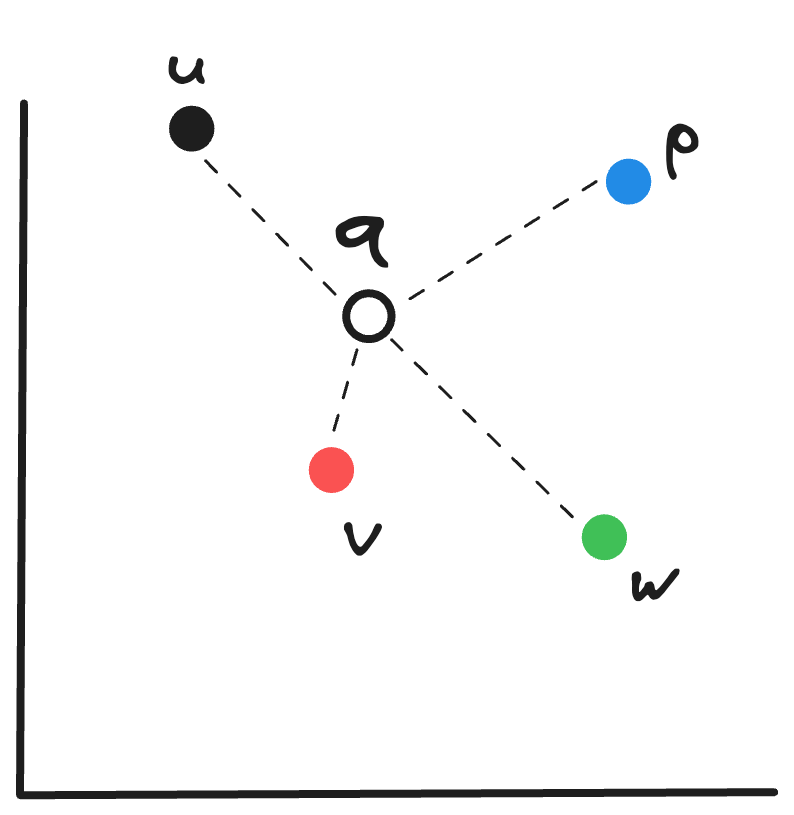
\includegraphics[width=0.45\linewidth]{figures/introduction-l2-knn.png}
%         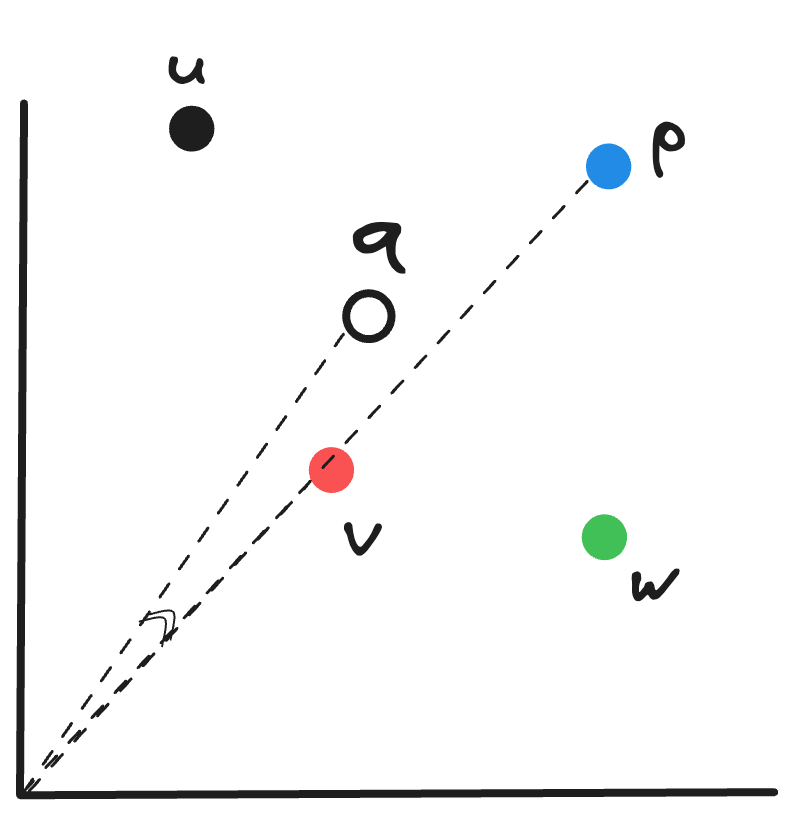
\includegraphics[width=0.45\linewidth]{figures/introduction-kmcs.png}
%     }
    
%     \subfloat[\textsc{Quora}-\textsc{AllMiniLM-l6-v2} (dense)]{
%         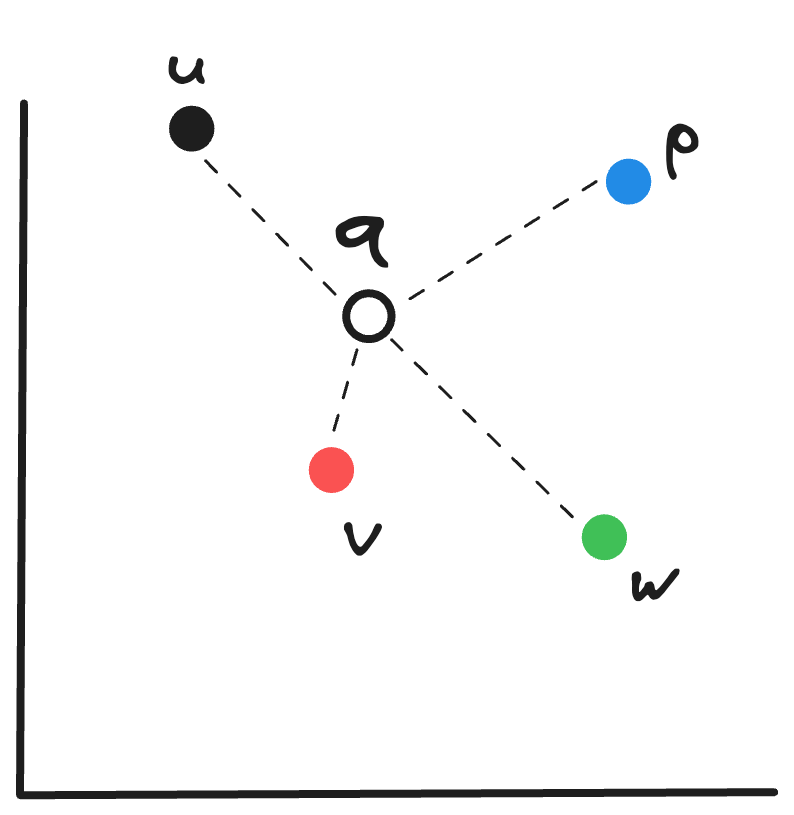
\includegraphics[width=0.45\linewidth]{figures/introduction-l2-knn.png}
%         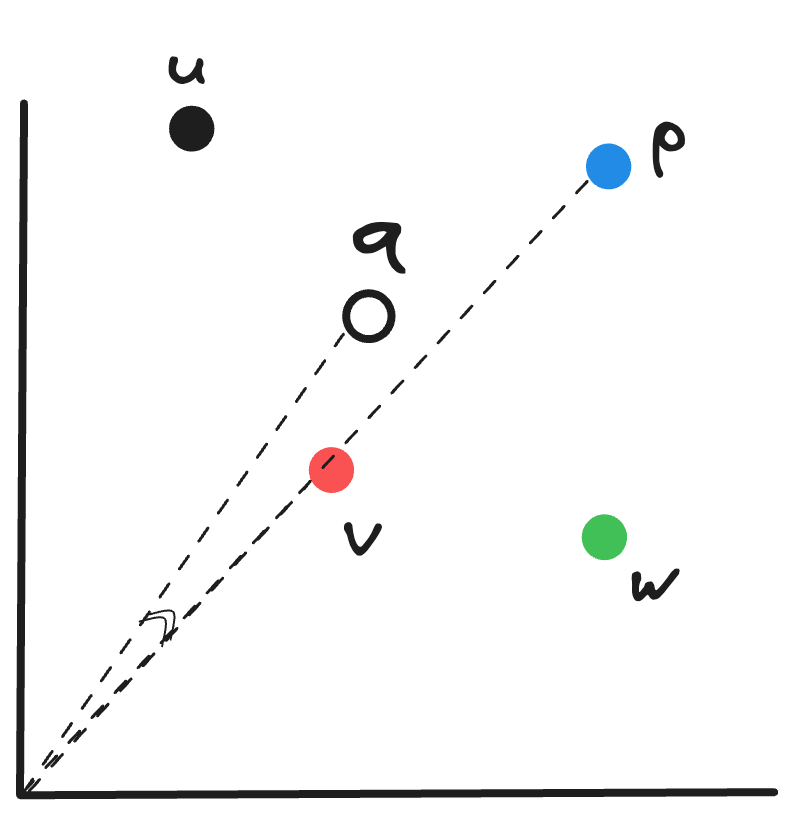
\includegraphics[width=0.45\linewidth]{figures/introduction-kmcs.png}
%     }
%     \caption{An empirical evaluation of the sketching methods
%     by~\cite{daliri2023sampling} (left) and~\cite{bruch2023sinnamon} (right)
%     on a sparse and non-negative collection (top row) and a dense vector collection (bottom row).
%     We retrieve the top-$k^\prime$ vectors using sketches, and count how many of them are
%     the true top-$10$ solutions, and plot the mean accuracy for each configuration of $k^\prime$.
%     For a description of the datasets, see Appendix~\ref{appendix:collections}.}
%     \label{figure:sketching:comparison}
% \end{figure}

\bibliographystyle{abbrvnat}
\bibliography{biblio}
